\documentclass[11pt,a4paper]{article}

\usepackage[T1]{fontenc}
\usepackage[utf8]{inputenc}
\IfFileExists{libertinus.sty}{\usepackage{libertinus}}{\usepackage{lmodern}}
\usepackage{microtype}
\usepackage[a4paper,margin=27mm,headheight=15pt]{geometry}
\usepackage{amsmath,amssymb,amsthm,mathtools}
% Canonical mathematical notation for active FabiusFunction LaTeX documents.
%
% This file is intentionally a plain TeX input rather than a LaTeX package.
% Every standalone document loads it by an explicit path relative to that
% document's directory; included fragments inherit the definitions from their
% root document.  Keep this file independent of document layout and metadata.
%
% Contract:
%   * one command has one mathematical meaning throughout the active corpus;
%   * names encode semantic roles rather than a document-local choice of letter;
%   * visually similar but differently normalized objects have different print;
%   * every command below is defined normatively in the notation catalogue.
%
% The active corpus excludes docs/archive/.  Historical sources may retain
% their original notation only inside an explicitly labelled quotation.

\makeatletter
\@ifundefined{mathbb}{%
  \PackageError{fabius-notation}{The amssymb package must be loaded first}%
    {Load amsmath and amssymb before inputting fabius-notation.tex.}%
}{}
\@ifundefined{operatorname}{%
  \PackageError{fabius-notation}{The amsmath package must be loaded first}%
    {Load amsmath before inputting fabius-notation.tex.}%
}{}
\makeatother

% Version stamp used by the catalogue and by static audits.
\newcommand{\FabiusNotationVersion}{2026-08-31}

% Number systems.  NaturalNumbers is explicitly the nonnegative convention.
\newcommand{\NaturalNumbers}{\mathbb{N}_{0}}
\newcommand{\PositiveIntegers}{\mathbb{N}_{>0}}
\newcommand{\IntegerNumbers}{\mathbb{Z}}
\newcommand{\RationalNumbers}{\mathbb{Q}}
\newcommand{\RealNumbers}{\mathbb{R}}
\newcommand{\ComplexNumbers}{\mathbb{C}}
\newcommand{\ExtendedRealNumbers}{\overline{\mathbb{R}}}

% The three principal Fabius--Rvachev functions.  Subscripts are deliberate:
% a bare F and a calligraphic F have several unrelated uses in the corpus.
\newcommand{\FabiusBounded}{F_{\mathrm{bd}}}
\newcommand{\FabiusGlobal}{F_{\mathrm{gl}}}
\newcommand{\FabiusQuantile}{Q_{F}}
\newcommand{\FabiusClampedQuantile}{Q_{F,\mathrm{cl}}}
\newcommand{\RvachevUp}{\operatorname{up}}

% Constants, elementary operators, and delimiters.
\newcommand{\EulerE}{\mathrm{e}}
\newcommand{\ImaginaryUnit}{\mathrm{i}}
\newcommand{\Differential}{\mathop{}\!\mathrm{d}}
\newcommand{\AbsoluteValue}[1]{\left\lvert #1\right\rvert}
\newcommand{\Norm}[1]{\left\lVert #1\right\rVert}
\newcommand{\Floor}[1]{\left\lfloor #1\right\rfloor}
\newcommand{\Ceiling}[1]{\left\lceil #1\right\rceil}
\newcommand{\FractionalPart}[1]{\left\{#1\right\}}
\newcommand{\PositivePart}[1]{\left(#1\right)_{+}}
\newcommand{\IndicatorOf}[1]{\mathbf{1}_{#1}}
\newcommand{\SetOf}[1]{\left\{#1\right\}}
\newcommand{\InnerProduct}[1]{\left\langle #1\right\rangle}
\newcommand{\CardinalityOf}[1]{\left\lvert #1\right\rvert}
\newcommand{\DefinitionEquals}{\mathrel{\coloneqq}}
\newcommand{\Sign}{\operatorname{sgn}}
\newcommand{\IdentityOperator}{\operatorname{id}}
\newcommand{\SpanOperator}{\operatorname{span}}
\newcommand{\TraceOperator}{\operatorname{tr}}
\newcommand{\RankOperator}{\operatorname{rank}}
\newcommand{\DiagonalOperator}{\operatorname{diag}}
\newcommand{\ResidueOperator}{\operatorname*{Res}}
\newcommand{\LeastCommonMultiple}{\operatorname{lcm}}
\newcommand{\OrderOperator}{\operatorname{ord}}
\newcommand{\PrincipalLogarithm}{\operatorname{Log}}
\newcommand{\FallingFactorial}[2]{\left(#1\right)^{\underline{#2}}}
\newcommand{\RisingFactorial}[2]{\left(#1\right)^{\overline{#2}}}

% Support, topology, convolution, and metric notation.
\newcommand{\SupportOperator}{\operatorname{supp}}
\newcommand{\SupportOf}[1]{\SupportOperator\!\left(#1\right)}
\newcommand{\TopologicalSupportOf}[1]{\operatorname{tsupp}\!\left(#1\right)}
\newcommand{\Convolution}{\mathbin{*}}
\newcommand{\MetricDistance}{\operatorname{dist}}
\newcommand{\TotalVariationDistance}{d_{\mathrm{TV}}}

% Probability.  Equality and convergence in law are not metric distance.
\newcommand{\Probability}{\mathbb{P}}
\newcommand{\Expectation}{\mathbb{E}}
\newcommand{\Variance}{\operatorname{Var}}
\newcommand{\Covariance}{\operatorname{Cov}}
\newcommand{\LawOperator}{\operatorname{Law}}
\newcommand{\LawOf}[1]{\LawOperator\!\left(#1\right)}
\newcommand{\EqualInLaw}{\mathrel{\overset{\mathrm{law}}{=}}}
\newcommand{\ConvergesInLaw}{\mathrel{\xrightarrow{\mathrm{law}}}}

% Fourier and integral transforms.  The printed labels expose normalization.
% FourierTwoPi uses exp(-2*pi*i*x*xi); FourierAngular uses exp(-i*x*omega).
\newcommand{\FourierTwoPi}[1]{\widehat{#1}_{\,2\pi}}
\newcommand{\FourierAngular}[1]{\widehat{#1}_{\,\mathrm{ang}}}
\newcommand{\LaplaceTransformSymbol}{\mathcal{L}}
\newcommand{\MellinTransformSymbol}{\mathcal{M}}
\newcommand{\LaplaceTransformOf}[1]{\LaplaceTransformSymbol\!\left[#1\right]}
\newcommand{\MellinTransformOf}[1]{\MellinTransformSymbol\!\left[#1\right]}
\newcommand{\MomentGeneratingFunction}[1]{M_{#1}}
\newcommand{\CharacteristicFunction}[1]{\varphi_{#1}}

% The two standard sinc functions must never share one symbol.
\newcommand{\SincRad}{\operatorname{sinc}_{\mathrm{rad}}}
\newcommand{\SincPi}{\operatorname{sinc}_{\pi}}

% Binary arithmetic and Thue--Morse notation.
\newcommand{\BinaryDigitSum}{\operatorname{wt}_{2}}
\newcommand{\ThueMorseSignSymbol}{\varepsilon}
\newcommand{\ThueMorseSign}[1]{\varepsilon_{#1}}
\newcommand{\PadicValuation}[1]{\nu_{#1}}
\newcommand{\TwoAdicValuation}{\nu_{2}}

% q-series notation.  Every base is an explicit argument.
\newcommand{\QPochhammer}[3]{\left(#1;#2\right)_{#3}}
\newcommand{\GaussianBinomial}[3]{%
  \genfrac{[}{]}{0pt}{}{#1}{#2}_{#3}%
}
\newcommand{\QInteger}[2]{\left[#1\right]_{#2}}

% Named special functions.
\newcommand{\Polylogarithm}{\operatorname{Li}}
\newcommand{\LambertW}{W}
\newcommand{\GammaFunction}{\Gamma}
\newcommand{\RiemannZeta}{\zeta}

% Asymptotics.  BigO and LittleO are operator tokens for existing formula
% grammar; prefer the At forms so that the limiting regime is printed.
\newcommand{\BigO}{\mathcal{O}}
\newcommand{\LittleO}{o}
\newcommand{\BigOAt}[2]{\mathcal{O}_{#2}\!\left(#1\right)}
\newcommand{\LittleOAt}[2]{o_{#2}\!\left(#1\right)}

\usepackage{bm}
\usepackage{booktabs,longtable,tabularx,array}
\usepackage{enumitem}
\usepackage{graphicx}
\usepackage{xcolor}
\usepackage{fancyhdr}
\usepackage{listings}
\usepackage{url}
\usepackage{hyperref}
\usepackage[nameinlink,capitalize,noabbrev]{cleveref}
\usepackage{caption}
\usepackage{subcaption}
\usepackage{float}
\usepackage{setspace}

\hypersetup{
  colorlinks=true,
  linkcolor=blue!45!black,
  citecolor=green!35!black,
  urlcolor=blue!55!black,
  pdftitle={Parameter-Flow, Gaussian, and Large-Deviation Frontiers for the q-Fabius--Rvachev Family},
  pdfauthor={OpenAI GPT-5.6 Pro},
  pdfsubject={Fabius function, Rvachev up-function, geometric uniform series, q-analogues, Edgeworth expansions, large deviations, Lambert W},
  pdfkeywords={Fabius function, Rvachev up-function, q-series, infinite sinc product, Bernoulli numbers, Lambert W, Edgeworth expansion, large deviations, convex order}
}

\pagestyle{fancy}
\fancyhf{}
\fancyhead[L]{\footnotesize q-Fabius--Rvachev frontiers}
\fancyhead[R]{\footnotesize \thepage}
\fancyfoot{}

\setlist[itemize]{leftmargin=*,topsep=3pt,itemsep=2pt}
\setlist[enumerate]{leftmargin=*,topsep=3pt,itemsep=2pt}
\setstretch{1.04}

\newtheorem{theorem}{Theorem}[section]
\newtheorem{proposition}[theorem]{Proposition}
\newtheorem{lemma}[theorem]{Lemma}
\newtheorem{corollary}[theorem]{Corollary}
\newtheorem{conjecture}[theorem]{Conjecture}
\newtheorem{problem}[theorem]{Problem}
\newtheorem{principle}[theorem]{Principle}
\theoremstyle{definition}
\newtheorem{definition}[theorem]{Definition}
\newtheorem{remark}[theorem]{Remark}
\newtheorem{example}[theorem]{Example}

\newcommand{\sinhc}{\operatorname{sinhc}}
\newcommand{\cx}{\preceq_{\mathrm{cx}}}
\newcommand{\eps}{\varepsilon}
\newcommand{\cL}{C_{\Lambda}}
\newcommand{\He}{H}


\lstdefinestyle{pythonstyle}{
  language=Python,
  basicstyle=\ttfamily\footnotesize,
  keywordstyle=\color{blue!60!black},
  commentstyle=\color{green!35!black},
  stringstyle=\color{red!50!black},
  breaklines=true,
  frame=single,
  showstringspaces=false,
  columns=fullflexible
}

\title{\bfseries Parameter-Flow, Gaussian, and Large-Deviation Frontiers\\[2mm]
for the $q$-Fabius--Rvachev Family}
\author{Research report prepared by OpenAI GPT-5.6 Pro}
\date{30 August 2026}

\begin{document}

\maketitle

\begin{abstract}
Let $U_0,U_1,\ldots$ be independent $\operatorname{Unif}[-1,1]$ variables and
\[
  X_q=(1-q)\sum_{j\ge0}q^jU_j,\qquad 0<q<1.
\]
At $q=1/2$ the density of $X_q$ is the standard centered Rvachev
$\RvachevUp$-function, and hence lies on the usual Fabius--Rvachev bridge.  The
current ProveIt corpus already contains an extensive theory of this family:
its infinite-sinc transform, Bernoulli cumulants, $q$-Pochhammer
factorizations, parameter limits, fixed-base endpoint asymptotics, finite
prefix transport, and a first Gaussian correction.  After a source-level
crosswalk against that corpus, this report develops a different parameter
layer.

First, for $0<r<s<1$ we construct an explicit probability kernel
$p_{r,s}$ whose generating function is
\[
  P_{r,s}(z)=\frac{1-s}{1-r}\frac{1-rz}{1-sz}.
\]
It transports the geometric coefficient profile at $r$ to that at $s$ and
forms a convolution cocycle.  A random tail shift with law $p_{r,s}$ gives an
explicit martingale coupling, proving the universal convex-order flow
$X_s\preceq_{\mathrm{cx}}X_r$.  The kernels are the increments of an
inhomogeneous compound-Poisson subordinator with geometric jump law.

Second, writing $q=\EulerE^{-\delta}$, we prove a full large-deviation principle at
speed $1/\delta$.  Its limiting scaled cumulant transform is
\[
 \Lambda(\theta)=\int_0^\infty
     \log\!\left(\frac{\sinh(\theta \EulerE^{-t})}{\theta \EulerE^{-t}}\right)\Differential t
 =\int_0^\theta\frac{\log(\sinh u/u)}{u}\Differential u,
\]
and the rate is $I=\Lambda^*$.  The finite-$q$ transform is an exact midpoint
Riemann sum.  Midpoint Euler--Maclaurin therefore yields an all-orders
expansion containing only even powers of $\delta$ and Bernoulli polynomials
at $1/2$; in particular
\[
 \Lambda_\delta(\theta)=\Lambda(\theta)
 -\frac{\delta^2\theta^2}{24}\Lambda''(\theta)+O(\delta^4).
\]
The rate has an explicit rational Taylor series at the origin and a new
Lambert-$W_{-1}$ boundary law as $x\uparrow1$.

Third, we prove a uniform all-orders Edgeworth expansion for the
\emph{continuous} limit $q\uparrow1$, valid after any fixed number of density
derivatives.  This is distinct from the discrete $\mathrm{Fup}_n$ Edgeworth
theorem already present in the repository.  Exact Bernoulli cumulants produce
the Hermite coefficients, and a geometric infinite-sinc tail lemma supplies
the global Fourier control.  Numerical experiments reproduce the predicted
orders $1,2,3,4$ and the midpoint orders $2,4$.  The report closes with a
moderate-deviation bridge, sharp saddlepoint and positivity conjectures, and
a formalization roadmap.  All theorem proofs here are paper-level arguments;
no claim of Lean verification is made.
\end{abstract}

\tableofcontents
\newpage

\section{Scope, corpus audit, and nonduplication boundary}
\label{sec:audit}

\subsection{What was compared}

The source tree under
\begin{center}
\url{https://github.com/VladimirReshetnikov/ProveIt/tree/main/Analysis/FabiusFunction/docs}
\end{center}
contains the expository Fabius and Rvachev documents, the Lean walkthrough,
archival material, the canonical semi-formalized frontier volume, and a large
set of current standalone drafts.  The working comparison used the live
source tree, the canonical frontier volume and its group READMEs, and the
global draft manifest dated 28--30 August 2026 \cite{ProveItDocs,ProveItManifest}.  The purpose of the comparison
was not merely to avoid repeated wording: it was to remove mathematical
layers whose main claims were already present under different titles.

The following table records the decisive exclusions and the boundary of the
present contribution.  ``New here'' always means \emph{not found in the live
repository crosswalk used for this report}; it is not an unqualified claim of
priority over all mathematical literature.

\begin{longtable}{p{0.25\textwidth}p{0.34\textwidth}p{0.32\textwidth}}
\toprule
Corpus layer & Already present & Layer developed here \\
\midrule
\endfirsthead
\toprule
Corpus layer & Already present & Layer developed here \\
\midrule
\endhead
Exponent- and $q$-series frontiers, Parts VI--VII
& The geometric family, infinite sinc products, exact Bernoulli cumulants,
$q$-Pochhammer structure, quantitative $q\uparrow1$ Gaussian convergence, and
the first characteristic correction
& A complete continuous-parameter Edgeworth hierarchy, uniform on $\RealNumbers$ and
after arbitrary fixed derivatives \\
\addlinespace
Finite-sinc transport, Part V
& Convex order, peakedness, stop-loss identities, and exact metrics along the
\emph{prefix index} $N$
& Convex order along the \emph{geometric parameter} $q$, with an explicit
tail-shift martingale and a compound-Poisson cocycle \\
\addlinespace
Atomic-function/Fup hierarchy
& A proved all-orders Edgeworth theorem for the discrete family
$\mathrm{Fup}_n$
& A separate theorem for $X_q$ as the continuous parameter $q\uparrow1$;
the triangular arrays and cumulant weights differ \\
\addlinespace
Fixed-base endpoint/Lambert theory
& Spatial endpoint asymptotics at fixed $q$ or fixed base, including
Lambert-$W_{-1}$ inversion and periodic transform terms
& A parameter-boundary large-deviation rate as $q\uparrow1$, whose own
$x\uparrow1$ saddle has a distinct Lambert-$W_{-1}$ law \\
\addlinespace
Shape, native orthogonal-polynomial, and noncommutative reports
& Strict log-concavity, native Jacobi/Hankel theory, free and Boolean
cumulants, and non-free-infinite-divisibility certificates
& Explicitly omitted after the final cross-check \\
\bottomrule
\end{longtable}

\subsection{Main claims of the report}

The central claims are the following.

\begin{enumerate}[label=\textbf{R\arabic*.}]
\item An exact coefficient kernel $p_{r,s}$, its cocycle, its
compound-Poisson generator, and an explicit martingale proof of
$X_s\preceq_{\mathrm{cx}}X_r$.
\item An all-orders midpoint Euler--Maclaurin expansion for the scaled
$q\uparrow1$ cumulant transform.
\item A G\"artner--Ellis large-deviation principle with an explicit integral
transform, rational central rate series, and Lambert-$W_{-1}$ edge inversion.
\item A differentiated, uniform, all-orders Edgeworth expansion for the
continuous geometric family.
\item Matching between central and large deviations, together with
saddlepoint, coefficient-positivity, and transseries conjectures.
\end{enumerate}

The constructions extend verbatim to many bounded seed distributions.  The
uniform seed is singled out because it is exactly the Fabius--Rvachev case
and because its cumulant transform is controlled by Bernoulli numbers.

\section{The geometric-uniform law and the Fabius--Rvachev point}
\label{sec:setup}

\subsection{Random series, transforms, and fixed point}

Let $U_0,U_1,\dots$ be independent variables with density
$\frac12\IndicatorOf{[-1,1]}$.  For $0<q<1$ define
\begin{equation}
  X_q=(1-q)\sum_{j=0}^{\infty}q^jU_j.
  \label{eq:Xq}
\end{equation}
The series converges absolutely almost surely, $\Expectation X_q=0$, and
$|X_q|\le1$.  Its distribution is the unique compactly supported solution of
\begin{equation}
  X_q\overset{d}= (1-q)U+qX_q',
  \label{eq:perpetuity}
\end{equation}
where $X_q'$ is an independent copy.  We use
\[
 \SincRad z=\frac{\sin z}{z},\qquad
 \sinhc z=\frac{\sinh z}{z},
\]
with their continuous values at zero.  The characteristic and moment
generating functions are
\begin{align}
 \phi_q(t)&=\Expectation \EulerE^{itX_q}
   =\prod_{j=0}^{\infty}\SincRad\bigl((1-q)q^jt\bigr),
   \label{eq:cf}\\
 M_q(t)&=\Expectation \EulerE^{tX_q}
   =\prod_{j=0}^{\infty}\sinhc\bigl((1-q)q^jt\bigr).
   \label{eq:mgf}
\end{align}
At $q=1/2$ the first product is
$\prod_{k\ge1}\SincRad(t/2^k)$, the standard Fourier transform of the centered
Rvachev $\RvachevUp$-function.  Thus $X_{1/2}$ is exactly the centered up-law; the
usual piecewise shift/reflection relation then connects its density to the
Fabius function \cite{Fabius1966,Rvachev1990,Arias2018}.

\subsection{Bernoulli cumulants}

Let $B_n$ denote the Bernoulli numbers with $B_2=1/6$.  Since
\begin{equation}
 \log\sinhc z
 =\sum_{m=1}^{\infty}
   \frac{2^{2m-1}B_{2m}}{m(2m)!}z^{2m},
 \qquad |z|<\pi,
 \label{eq:logsinhc-series}
\end{equation}
the even cumulants of $U$ and $X_q$ are
\begin{align}
 \kappa_{2m}(U)&=\frac{2^{2m-1}B_{2m}}{m},
 \label{eq:uniform-cumulants}\\
 \kappa_{2m}(X_q)&=\frac{2^{2m-1}B_{2m}}{m}
     \frac{(1-q)^{2m}}{1-q^{2m}},
 \qquad \kappa_{2m+1}(X_q)=0.
 \label{eq:Xq-cumulants}
\end{align}
In particular
\begin{equation}
 \sigma_q^2:=\Variance(X_q)=\frac{1-q}{3(1+q)}.
 \label{eq:variance}
\end{equation}
The moments are complete Bell polynomials in the cumulants \cite{Comtet}, so every even
moment is a rational function of $q$ with Bernoulli input.  This exact
cumulant layer is part of the established corpus; our use of it below is to
build the new parameter asymptotics.

\subsection{The natural small parameter}

Set
\begin{equation}
 q=\EulerE^{-\delta},\qquad \delta=-\log q.
 \label{eq:delta}
\end{equation}
Then
\begin{equation}
 1-q=\delta s_\delta \EulerE^{-\delta/2},
 \qquad
 s_\delta:=\frac{2\sinh(\delta/2)}{\delta}
 =1+\frac{\delta^2}{24}+\frac{\delta^4}{1920}+O(\delta^6).
 \label{eq:sdelta}
\end{equation}
This exact half-step factorization is the source of the midpoint
Euler--Maclaurin cancellation in \cref{sec:midpoint}.  Notice also
\begin{equation}
 \sigma_q^2=\frac13\tanh\frac{\delta}{2}
 =\frac{\delta}{6}-\frac{\delta^3}{72}
   +\frac{\delta^5}{720}+O(\delta^7).
 \label{eq:variance-delta}
\end{equation}
Thus the unstandardized law collapses to zero at scale $\sqrt\delta$, while
its standardized form tends to a Gaussian.

\section{An exact parameter-flow kernel and martingale transport}
\label{sec:transport}

The finite-prefix transport theory already in the corpus orders successive
truncations.  Here the number of factors is infinite and the parameter itself
moves.  The key observation is that the geometric coefficient profile admits
an exact stochastic factorization.

\subsection{Coefficient cocycle}

Write
\begin{equation}
 a_j(q)=(1-q)q^j,
 \qquad
 A_q(z)=\sum_{j\ge0}a_j(q)z^j=\frac{1-q}{1-qz}.
 \label{eq:coefficient-pgf}
\end{equation}

\begin{theorem}[Parameter-flow kernel]
\label{thm:kernel}
For $0<r<s<1$, define a probability mass function on $\NaturalNumbers$ by
\begin{equation}
 p_{r,s}(0)=\frac{1-s}{1-r},\qquad
 p_{r,s}(k)=\frac{(s-r)(1-s)}{1-r}s^{k-1},\quad k\ge1.
 \label{eq:prs}
\end{equation}
Its probability generating function is
\begin{equation}
 P_{r,s}(z)=\sum_{k\ge0}p_{r,s}(k)z^k
 =\frac{1-s}{1-r}\frac{1-rz}{1-sz}.
 \label{eq:Prs}
\end{equation}
The geometric coefficient profiles satisfy
\begin{equation}
 a(s)=p_{r,s}*a(r),
 \qquad A_s(z)=P_{r,s}(z)A_r(z),
 \label{eq:coefficient-convolution}
\end{equation}
and the kernels form the convolution cocycle
\begin{equation}
 p_{r,t}=p_{s,t}*p_{r,s},
 \qquad 0<r<s<t<1.
 \label{eq:cocycle}
\end{equation}
\end{theorem}

\begin{proof}
The coefficients in \eqref{eq:prs} are nonnegative and
\[
 p_{r,s}(0)+\sum_{k\ge1}p_{r,s}(k)
 =\frac{1-s}{1-r}+\frac{s-r}{1-r}=1.
\]
Dividing the two rational functions in \eqref{eq:coefficient-pgf} gives
\[
 \frac{A_s(z)}{A_r(z)}
 =\frac{1-s}{1-r}\frac{1-rz}{1-sz},
\]
whose geometric-series expansion is exactly \eqref{eq:prs}.  This proves
\eqref{eq:coefficient-convolution}.  The cocycle follows immediately from
$P_{r,t}=A_t/A_r=(A_t/A_s)(A_s/A_r)$.
\end{proof}

\subsection{Compound-Poisson interpretation}

The cocycle is not merely algebraic.  Differentiating its logarithm in the
upper parameter gives
\begin{align}
 \frac{\partial}{\partial s}\log P_{r,s}(z)
 &=\frac{z}{1-sz}-\frac{1}{1-s}
 \notag\\
 &=\sum_{k\ge1}s^{k-1}(z^k-1).
 \label{eq:levy-generator}
\end{align}
Consequently
\begin{equation}
 P_{r,s}(z)=
 \exp\left\{\int_r^s\sum_{k\ge1}u^{k-1}(z^k-1)\Differential u\right\}.
 \label{eq:compound-poisson-pgf}
\end{equation}

\begin{proposition}[Inhomogeneous geometric-jump subordinator]
\label{prop:subordinator}
There exists an increasing process $(N_q)_{0<q<1}$ with independent
increments such that $N_s-N_r$ has law $p_{r,s}$.  At parameter value $u$,
jumps occur with total intensity $(1-u)^{-1}\Differential u$, and conditional on a
jump the size has geometric law
\begin{equation}
 \Probability\{J=k\mid u\}=(1-u)u^{k-1},\qquad k\ge1.
 \label{eq:geometric-jumps}
\end{equation}
\end{proposition}

\begin{proof}
Equation \eqref{eq:compound-poisson-pgf} is the L\'evy--Khintchine formula
for an inhomogeneous compound-Poisson process with jump intensity measure
$u^{k-1}\Differential u$ at size $k$.  Summing over $k$ gives total rate
$\sum_{k\ge1}u^{k-1}=(1-u)^{-1}$, and normalization gives
\eqref{eq:geometric-jumps}.
\end{proof}

The expected number of jumps between $r$ and $s$ is
$\log((1-r)/(1-s))$.  Thus the apparently static operation of making the
coefficient sequence more diffuse is governed by a simple pure-jump flow.

\subsection{Explicit martingale coupling}

The kernel acts by random shifts of the independent environment.  This gives
a direct convex-order proof, stronger than a comparison of finitely many
moments.

\begin{theorem}[Tail-shift martingale transport]
\label{thm:martingale-transport}
Let $V_0,V_1,\ldots$ be iid integrable real random variables and define
\begin{equation}
 X_q^{(V)}=(1-q)\sum_{j\ge0}q^jV_j.
 \label{eq:general-seed}
\end{equation}
For $0<r<s<1$, let $N$ be independent of the sequence and have law
$p_{r,s}$.  Put
\begin{equation}
 Y_{r,s}=\sum_{j\ge0}a_j(r)V_{j+N}.
 \label{eq:Yrs}
\end{equation}
Then
\begin{equation}
 Y_{r,s}\overset d=X_r^{(V)},
 \qquad
 \Expectation\!\left[Y_{r,s}\mid V_0,V_1,\ldots\right]=X_s^{(V)}.
 \label{eq:martingale-coupling}
\end{equation}
Consequently
\begin{equation}
 X_s^{(V)}\preceq_{\mathrm{cx}}X_r^{(V)}.
 \label{eq:convex-order}
\end{equation}
\end{theorem}

\begin{proof}
For every fixed $n$, the tail $(V_n,V_{n+1},\ldots)$ has the same joint law
as the original iid sequence, hence the conditional-on-$N=n$ variable in
\eqref{eq:Yrs} has law $X_r^{(V)}$.  Thus $Y_{r,s}\overset d=X_r^{(V)}$.
Conditioning instead on the entire environment and using Tonelli's theorem
for the absolutely summable coefficients gives
\begin{align*}
 \Expectation[Y_{r,s}\mid(V_j)_{j\ge0}]
 &=\sum_{n\ge0}p_{r,s}(n)\sum_{j\ge0}a_j(r)V_{j+n}\\
 &=\sum_{k\ge0}\left(\sum_{n=0}^{k}p_{r,s}(n)a_{k-n}(r)\right)V_k\\
 &=\sum_{k\ge0}a_k(s)V_k
 =X_s^{(V)},
\end{align*}
where the penultimate equality is \eqref{eq:coefficient-convolution}.
Therefore $X_s^{(V)}$ is the conditional expectation of a variable having
law $X_r^{(V)}$.  Jensen's inequality yields
$\Expectation\Phi(X_s^{(V)})\le\Expectation\Phi(X_r^{(V)})$ for every convex $\Phi$ for which
the expectations exist, which is exactly convex order.
\end{proof}

\begin{corollary}[Stop-loss and moment inequalities]
\label{cor:stoploss}
For $0<r<s<1$ and every $t\in\RealNumbers$,
\begin{equation}
 \Expectation(X_s-t)_+\le \Expectation(X_r-t)_+.
 \label{eq:stoploss}
\end{equation}
If the seed is centered and has finite variance, then
\begin{equation}
 \Variance(X_q^{(V)})=\Variance(V)\frac{1-q}{1+q},
 \label{eq:general-variance}
\end{equation}
and this variance is strictly decreasing unless $V$ is degenerate.  All
even convex moments that exist are nonincreasing in $q$.
\end{corollary}

\begin{remark}[Why the proof is genuinely infinite-dimensional]
The right shift of an infinite coefficient sequence is not a finite
permutation.  Nevertheless every shifted iid tail produces exactly the same
weighted-sum law.  Averaging over the shift kernel therefore supplies the
martingale directly and bypasses finite-dimensional approximation.  The
finite-prefix convex-order chain in the repository and the parameter flow
\eqref{eq:convex-order} are complementary rather than duplicate statements.
\end{remark}

\section{The scaled cumulant transform as a midpoint \texorpdfstring{$q$}{q}-integral}
\label{sec:midpoint}

\subsection{Exact half-step representation}

For the uniform seed set
\begin{equation}
 g(z)=\log\sinhc z=\log\frac{\sinh z}{z}.
 \label{eq:gdef}
\end{equation}
The scaled cumulant generating function at large-deviation speed
$1/\delta$ is
\begin{equation}
 \Lambda_\delta(\theta)
 :=\delta\log\Expectation\exp\!\left(\frac{\theta X_{\EulerE^{-\delta}}}{\delta}\right).
 \label{eq:scaled-cgf}
\end{equation}
Using \eqref{eq:sdelta}, the $j$th argument of $g$ is
\[
 \frac{\theta(1-\EulerE^{-\delta})\EulerE^{-j\delta}}{\delta}
 =\theta s_\delta \EulerE^{-(j+1/2)\delta}.
\]
Hence the exact identity
\begin{equation}
 \boxed{\quad
 \Lambda_\delta(\theta)
 =\delta\sum_{j=0}^{\infty}
 g\!\left(\theta s_\delta \EulerE^{-(j+1/2)\delta}\right).
 \quad}
 \label{eq:midpoint-sum}
\end{equation}
This is a midpoint Riemann sum on the logarithmic scale.  It is the reason the
first correction is $O(\delta^2)$ rather than $O(\delta)$.

\subsection{Limit transform}

\begin{theorem}[Limiting scaled cumulant transform]
\label{thm:lambda-limit}
Uniformly for $\theta$ in compact subsets of $\RealNumbers$,
\begin{equation}
 \Lambda_\delta(\theta)\longrightarrow
 \Lambda(\theta):=\int_0^\infty g(\theta \EulerE^{-t})\Differential t
 =\int_0^\theta\frac{g(u)}{u}\Differential u.
 \label{eq:Lambda}
\end{equation}
The function $\Lambda$ is even, real analytic, and strictly convex, with
\begin{align}
 \Lambda'(\theta)&=\frac{1}{\theta}
    \log\frac{\sinh\theta}{\theta},
 \label{eq:Lambda-prime}\\
 \Lambda''(\theta)&=
 \frac{\theta\coth\theta-
       \log(\sinh\theta/\theta)-1}{\theta^2}>0,
 \label{eq:Lambda-second}\\
 \Lambda'(\RealNumbers)&=(-1,1).
 \label{eq:gradient-range}
\end{align}
At the origin,
\begin{equation}
 \Lambda(\theta)=
 \sum_{m\ge1}
 \frac{2^{2m-2}B_{2m}}{m^2(2m)!}\theta^{2m}
 =\frac{\theta^2}{12}-\frac{\theta^4}{720}
  +\frac{\theta^6}{17010}-\cdots.
 \label{eq:Lambda-Bernoulli}
\end{equation}
\end{theorem}

\begin{proof}
For bounded $\theta$, the summand in \eqref{eq:midpoint-sum} is smooth and
bounded by $C\theta^2\EulerE^{-2t}$ after the identification
$t=(j+1/2)\delta$.  Riemann-sum convergence is therefore uniform on compact
$\theta$-sets and yields the first integral in \eqref{eq:Lambda}.  The change
of variables $u=\theta \EulerE^{-t}$ yields the second.  Differentiation under the
integral is justified by the same exponential envelope.  Since
$g$ is the cumulant generating function of a nondegenerate uniform variable,
$g''(u)>0$; therefore
\[
 \Lambda''(\theta)=\int_0^\infty \EulerE^{-2t}g''(\theta \EulerE^{-t})\Differential t>0.
\]
The explicit formulas follow by differentiating the second integral.  Finally
$g(\theta)=\theta-\log(2\theta)+O(\EulerE^{-2\theta})$ as
$\theta\to+\infty$, so $\Lambda'(\theta)=g(\theta)/\theta\to1$;
oddness gives the lower endpoint.  Integrating \eqref{eq:logsinhc-series}
termwise gives \eqref{eq:Lambda-Bernoulli}.
\end{proof}

\subsection{All-orders midpoint Euler--Maclaurin expansion}

Let $B_n(x)$ be the Bernoulli polynomials and let
$D=\theta\frac{\Differential}{\Differential\theta}$ be the Euler operator.

\begin{theorem}[All-order midpoint expansion]
\label{thm:midpoint-EM}
For every integer $N\ge1$ and every compact $K\subset\RealNumbers$,
\begin{align}
 \Lambda_\delta(\theta)
 &=\Lambda(\theta s_\delta)
 +\sum_{m=1}^{N-1}
   \frac{B_{2m}(1/2)}{(2m)!}\delta^{2m}
   D^{2m-1}g(\theta s_\delta)
 +O_{K,N}(\delta^{2N})
 \label{eq:EM-all-orders}
\end{align}
uniformly for $\theta\in K$.  In particular the expansion contains only
even powers of $\delta$.  The first two nontrivial terms are
\begin{align}
 \Lambda_\delta(\theta)
 &=\Lambda(\theta)
 -\frac{\delta^2\theta^2}{24}\Lambda''(\theta)
 +\delta^4 C_4(\theta)+O_K(\delta^6),
 \label{eq:Lambda-two-corrections}\\
 C_4(\theta)
 &=\frac{7D^3g-10D^2g+5Dg-2g}{5760}(\theta).
 \label{eq:C4}
\end{align}
\end{theorem}

\begin{proof}
For
$f_{\delta,\theta}(t)=g(\theta s_\delta \EulerE^{-t})$, all derivatives decay
exponentially as $t\to\infty$, uniformly for $\theta$ in a compact set.
The midpoint Euler--Maclaurin formula \cite{Olver} gives
\begin{equation}
 \delta\sum_{j\ge0}f_{\delta,\theta}((j+1/2)\delta)
 =\int_0^\infty f_{\delta,\theta}(t)\Differential t
 -\sum_{m=1}^{N-1}
   \frac{B_{2m}(1/2)}{(2m)!}\delta^{2m}
   f_{\delta,\theta}^{(2m-1)}(0)
 +O_{K,N}(\delta^{2N}).
 \label{eq:midpoint-EM-proof}
\end{equation}
The integral is $\Lambda(\theta s_\delta)$, while
$f^{(2m-1)}(0)=-D^{2m-1}g(\theta s_\delta)$, giving
\eqref{eq:EM-all-orders}.  The vanishing
$B_{2m+1}(1/2)=0$ explains the even-power structure.

For the first correction, use $B_2(1/2)=-1/12$ and
$s_\delta=1+\delta^2/24+O(\delta^4)$:
\[
 \frac{\delta^2}{24}\bigl(g-Dg\bigr)
 =-\frac{\delta^2\theta^2}{24}\Lambda''(\theta).
\]
Expanding one order further and using
$B_4(1/2)=7/240$ gives \eqref{eq:C4}.
\end{proof}

\begin{remark}[A q-calculus reading]
Equation \eqref{eq:midpoint-sum} is a logarithmic Jackson-type sum whose mesh
is $\delta=-\log q$, but the exact factor $s_\delta$ centers the sampling at
half steps.  The resulting coefficients are Bernoulli polynomials at
$1/2$, not merely Bernoulli numbers at zero.  This provides a direct bridge
between the repository's $q$-product layer and its Bernoulli/Euler--Maclaurin
layer \cite{GasperRahman}.
\end{remark}

\section{A large-deviation principle as \texorpdfstring{$q\uparrow1$}{q tends to 1}}
\label{sec:LDP}

\subsection{The rate function}

\begin{theorem}[Large-deviation principle]
\label{thm:LDP}
The family $X_{\EulerE^{-\delta}}$ satisfies a large-deviation principle on $\RealNumbers$
with speed $1/\delta$ and good rate function
\begin{equation}
 I(x)=\sup_{\theta\in\RealNumbers}\{\theta x-\Lambda(\theta)\}.
 \label{eq:rate-Legendre}
\end{equation}
The function $I$ is even, strictly convex on $(-1,1)$, satisfies $I(0)=0$,
and is infinite for $|x|\ge1$.  For $|x|<1$, let $\theta_x$ be the unique
solution of
\begin{equation}
 x=\Lambda'(\theta_x)
 =\frac1{\theta_x}\log\frac{\sinh\theta_x}{\theta_x}.
 \label{eq:saddle-equation}
\end{equation}
Then
\begin{equation}
 I(x)=\theta_xx-\Lambda(\theta_x),
 \qquad I'(x)=\theta_x,
 \qquad I''(x)=\frac1{\Lambda''(\theta_x)}.
 \label{eq:rate-parametric}
\end{equation}
\end{theorem}

\begin{proof}
The scaled logarithmic moment generating functions are exactly
$\Lambda_\delta$ in \eqref{eq:scaled-cgf}, and
\cref{thm:lambda-limit} gives pointwise convergence to the finite,
differentiable function $\Lambda$ on all of $\RealNumbers$.  Since every
$X_{\EulerE^{-\delta}}$ is supported on the common compact interval $[-1,1]$,
exponential tightness is automatic.  The G\"artner--Ellis theorem \cite{Ellis1984,DemboZeitouni} therefore
gives the LDP with Legendre transform \eqref{eq:rate-Legendre}.  Strict
convexity and \eqref{eq:gradient-range} give the unique saddle and the
parametric identities.  Outside $[-1,1]$ the rate is infinite by support.
At $x=1$,
$\theta-\Lambda(\theta)\to\infty$ by the asymptotic expansion proved in
\cref{thm:Lambert-edge}; hence $I(1)=\infty$, and similarly at $-1$.
\end{proof}

Thus for regular sets $A$ the logarithmic probability scale is
\begin{equation}
 \Probability\{X_q\in A\}
 =\exp\left[-\frac{\inf_{x\in A}I(x)+o(1)}{-\log q}\right].
 \label{eq:LDP-heuristic}
\end{equation}
This is a parameter-concentration law, not the fixed-$q$ spatial endpoint
asymptotic already developed in the corpus.

\subsection{Central rate series}

The inverse saddle map in \eqref{eq:saddle-equation} is analytic at zero.
Series reversion gives
\begin{align}
 \theta_x={}&6x+\frac{36}{5}x^3+\frac{1656}{175}x^5
 +\frac{9504}{875}x^7+\frac{709344}{67375}x^9
 +\frac{18086976}{1990625}x^{11}
 +O(x^{13}),
 \label{eq:theta-center-series}\\
 I(x)={}&3x^2+\frac95x^4+\frac{276}{175}x^6
 +\frac{1188}{875}x^8+\frac{354672}{336875}x^{10}
 +\frac{1507248}{1990625}x^{12}
 +O(x^{14}).
 \label{eq:I-center-series}
\end{align}
All displayed coefficients are positive.  The companion symbolic script
checks positivity through the $x^{16}$ coefficient.

\begin{conjecture}[Positivity of the rate series]
\label{conj:rate-positive}
Every coefficient after the constant term in the Taylor expansion
$I(x)=\sum_{n\ge1}c_nx^{2n}$ is strictly positive.
\end{conjecture}

This is stronger than convexity.  A proof may require showing that the inverse
of $g(\theta)/\theta$ belongs to a positivity-preserving class, perhaps after
a Stieltjes or Pick transform.  The Bernoulli signs in \eqref{eq:Lambda-Bernoulli}
make coefficient positivity far from formal.

\begin{figure}[H]
\centering
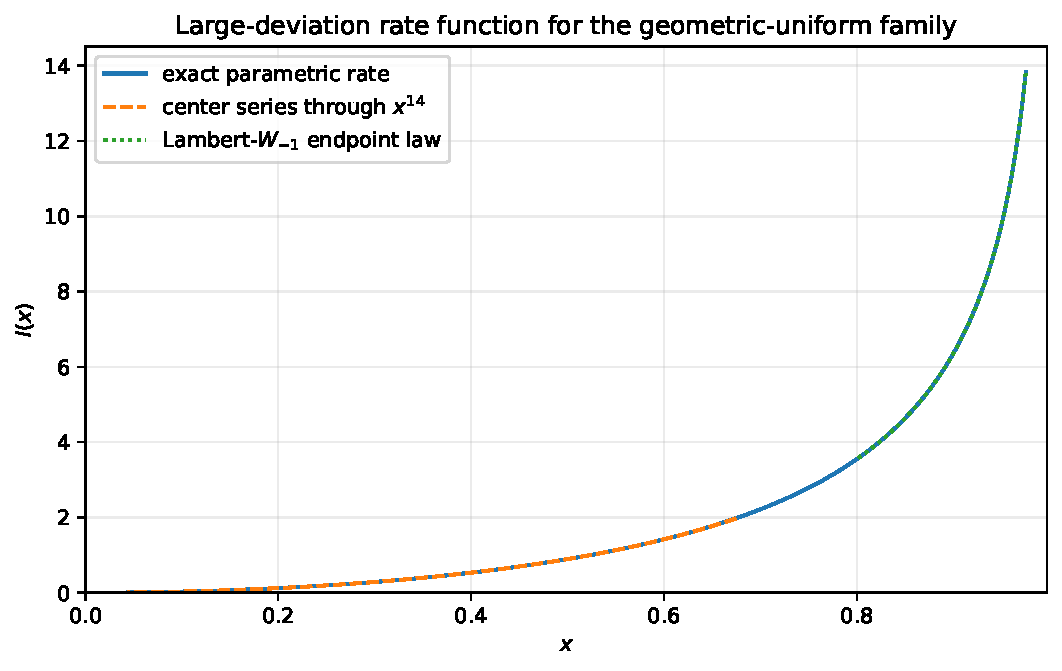
\includegraphics[width=0.92\textwidth]{figures/rate_function_lambert.pdf}
\caption{The exact parametric rate $I(x)$, its rational center expansion, and
the Lambert-$W_{-1}$ boundary approximation.  The latter is already visually
indistinguishable from the exact curve for $x\gtrsim0.8$.}
\label{fig:rate}
\end{figure}

\section{Lambert-\texorpdfstring{$W_{-1}$}{W(-1)} behavior at the rate boundary}
\label{sec:Lambert}

The fixed-base Fabius endpoint theory uses Lambert $W$ to invert flat spatial
tails.  The rate function develops a second, conceptually different Lambert
mechanism: the saddle parameter diverges as the deviation level approaches
the fixed support boundary.

\subsection{Asymptotics of the limiting transform}

For $u>0$,
\begin{equation}
 g(u)=u-\log(2u)+\log(1-\EulerE^{-2u}).
 \label{eq:g-large}
\end{equation}
Define the convergent constant
\begin{equation}
 \cL=
 \int_0^1\frac{\log(\sinh u/u)}{u}\Differential u-1
 +\int_1^\infty\frac{\log(1-\EulerE^{-2u})}{u}\Differential u.
 \label{eq:CLambda}
\end{equation}
Numerically,
\begin{equation}
 \cL=-0.96892042396303131827115715418362428628\ldots.
 \label{eq:CLambda-value}
\end{equation}

\begin{theorem}[Transform and saddle endpoint]
\label{thm:Lambert-edge}
As $\theta\to+\infty$,
\begin{align}
 \Lambda(\theta)
 &=\theta-\frac12(\log\theta)^2
   -(\log2)\log\theta+\cL
   +O\!\left(\frac{\EulerE^{-2\theta}}{\theta}\right),
 \label{eq:Lambda-large}\\
 1-\Lambda'(\theta)
 &=\frac{\log(2\theta)}{\theta}
   +O\!\left(\frac{\EulerE^{-2\theta}}{\theta}\right).
 \label{eq:Lambda-prime-large}
\end{align}
Let $\eta=1-x\downarrow0$ and
\begin{equation}
 \theta_0(\eta)=-\frac1\eta W_{-1}(-\eta/2).
 \label{eq:theta-Lambert}
\end{equation}
Then the exact saddle satisfies
\begin{equation}
 \theta_{1-\eta}=\theta_0(\eta)
 \left(1+O\!\left(\frac{\EulerE^{-2\theta_0(\eta)}}{\log\theta_0(\eta)}\right)\right),
 \label{eq:theta-Lambert-error}
\end{equation}
and, with $L_\eta=\log\theta_0(\eta)$,
\begin{equation}
 I(1-\eta)
 =\frac12L_\eta^2+(\log2-1)L_\eta
   -\log2-\cL+o(1).
 \label{eq:I-Lambert}
\end{equation}
\end{theorem}

\begin{proof}
Integrate \eqref{eq:g-large} from $1$ to $\theta$.  The elementary terms give
$\theta-\frac12(\log\theta)^2-(\log2)\log\theta$, while the two convergent
remainders combine exactly into \eqref{eq:CLambda}; the unintegrated tail is
$O(\EulerE^{-2\theta}/\theta)$.  Dividing \eqref{eq:g-large} by $\theta$ gives
\eqref{eq:Lambda-prime-large}.

The saddle equation becomes
\begin{equation}
 \eta\theta=\log(2\theta)-\log(1-\EulerE^{-2\theta}).
 \label{eq:edge-saddle-exact}
\end{equation}
Dropping the exponentially small last term yields
$\eta\theta=\log(2\theta)$, equivalent to
$(-\eta\theta)\EulerE^{-\eta\theta}=-\eta/2$.  The diverging positive solution is
\eqref{eq:theta-Lambert} on branch $W_{-1}$ \cite{Corless1996}.  A mean-value estimate in
\eqref{eq:edge-saddle-exact} gives \eqref{eq:theta-Lambert-error}.  Finally
substitute $x=1-\eta$, use
$\eta\theta=\log(2\theta)+o(1)$, and subtract \eqref{eq:Lambda-large} from
$\theta x$.
\end{proof}

\begin{remark}[Double logarithmic geometry]
The standard branch expansion gives
\[
 -W_{-1}(-\eta/2)
 =\log(2/\eta)+\log\log(2/\eta)+o(1),
\]
and consequently
\[
 L_\eta=\log(1/\eta)+\log\log(1/\eta)
 +o(\log\log(1/\eta)).
\]
Thus the rate diverges primarily like $\tfrac12\log^2(1/\eta)$,
with a forced $\log(1/\eta)\log\log(1/\eta)$ correction.  This is the parameter-LDP
counterpart of the log-squared endpoint structures elsewhere in the
Fabius--Rvachev theory.
\end{remark}

\section{Uniform all-orders Edgeworth expansion for \texorpdfstring{$q\uparrow1$}{q tends to 1}}
\label{sec:Edgeworth}

\subsection{Standardized infinite-sinc product}

Set
\begin{equation}
 Z_q=\frac{X_q}{\sigma_q},
 \qquad b_q=\frac{1-q}{\sigma_q}=\sqrt{3(1-q^2)}.
 \label{eq:Zq-bq}
\end{equation}
Then
\begin{equation}
 \chi_q(t):=\Expectation \EulerE^{itZ_q}
 =\prod_{j\ge0}\SincRad(b_qq^jt).
 \label{eq:standardized-cf}
\end{equation}
Let $\lambda_n(q)$ be the standardized cumulants of $Z_q$.  From
\eqref{eq:Xq-cumulants}, for $m\ge2$,
\begin{align}
 \lambda_{2m}(q)
 &=\frac{3^m2^{2m-1}B_{2m}}{m}
   \frac{(1-q^2)^m}{1-q^{2m}}
 \label{eq:lambda-q}\\
 &=\frac{3^m2^{3m-2}B_{2m}}{m}
   \frac{\sinh^m\delta}{\sinh(m\delta)},
 \qquad q=\EulerE^{-\delta}.
 \label{eq:lambda-delta}
\end{align}
Therefore $\lambda_{2m}=O(\delta^{m-1})$.  The first values are
\begin{align}
 \lambda_4&=-\frac65\tanh\delta
 =-\frac65\delta+\frac25\delta^3+O(\delta^5),
 \label{eq:lambda4}\\
 \lambda_6&=\frac{64}{7}\delta^2-\frac{64}{7}\delta^4+O(\delta^6),
 \label{eq:lambda6}\\
 \lambda_8&=-\frac{864}{5}\delta^3+\frac{1728}{5}\delta^5+O(\delta^7).
 \label{eq:lambda8}
\end{align}

\subsection{Weighted Hermite polynomial}

Let $H_n$ denote the probabilists' Hermite polynomials,
$\phi(x)=(2\pi)^{-1/2}\EulerE^{-x^2/2}$, and let a multi-index
$\bm{k}=(k_2,k_3,\ldots)$ have weight
\begin{equation}
 \BinaryDigitSum(\bm{k})=\sum_{m\ge2}(m-1)k_m,
 \qquad
 |\bm{k}|_*=\sum_{m\ge2}mk_m.
 \label{eq:edgeworth-weight}
\end{equation}
For $R\ge0$ define
\begin{equation}
 \mathcal E_{R,q}(x)=
 \sum_{\BinaryDigitSum(\bm{k})\le R}
 H_{2|\bm{k}|_*}(x)
 \prod_{m\ge2}\frac1{k_m!}
 \left(\frac{\lambda_{2m}(q)}{(2m)!}\right)^{k_m}.
 \label{eq:edgeworth-polynomial}
\end{equation}
Only finitely many indices contribute.  Keeping exact finite-$q$ cumulants is
useful: it automatically resums many higher powers of $\delta$.

\subsection{Global Fourier bounds}

\begin{lemma}[Geometric infinite-sinc tails]
\label{lem:sinc-tail}
Fix $q_0\in(0,1)$ and an integer $L\ge0$.  There exist positive constants
$c,C_L$ such that for $q_0\le q<1$,
\begin{equation}
 |\chi_q(t)|\le
 \begin{cases}
   \EulerE^{-ct^2},& |t|\le b_q^{-1},\\[1mm]
   C_L\exp\!\left(-\dfrac{c}{1-q}\right)
   (1+b_q|t|)^{-L},& |t|\ge b_q^{-1}.
 \end{cases}
 \label{eq:sinc-tail-bound}
\end{equation}
\end{lemma}

\begin{proof}
Choose $c_0>0$ such that
$|\SincRad u|\le \EulerE^{-c_0u^2}$ for $|u|\le1$.  If
$|t|\le b_q^{-1}$, every factor lies in that range and
\[
 |\chi_q(t)|\le
 \exp\left[-c_0b_q^2t^2\sum_{j\ge0}q^{2j}\right]
 =\EulerE^{-3c_0t^2}.
\]
For $|t|>b_q^{-1}$, choose $n$ so that
$b_qq^n|t|\le1<b_qq^{n-1}|t|$.  The product of factors with $j\ge n$ is at
most
\[
 \exp\left[-c_0b_q^2t^2\frac{q^{2n}}{1-q^2}\right]
 \le \exp\left[-\frac{c_0q_0^2}{1-q^2}\right],
\]
which is bounded by $\EulerE^{-c/(1-q)}$.  On the far part of the tail, the first
$L$ factors also satisfy $|\SincRad u|\le|u|^{-1}$ and supply the stated
polynomial decay.  The bounded transition interval is absorbed into $C_L$.
\end{proof}

\subsection{The differentiated theorem}

\begin{theorem}[Continuous-parameter Edgeworth expansion]
\label{thm:Edgeworth}
Let $f_q$ be the density of $Z_q$.  For every pair of nonnegative integers
$R$ and $r$, there exist $q_{R,r}<1$ and $C_{R,r}<\infty$ such that
\begin{equation}
 \sup_{x\in\RealNumbers}
 \left|
 f_q^{(r)}(x)-
 \frac{\Differential^r}{\Differential x^r}
 \bigl[\phi(x)\mathcal E_{R,q}(x)\bigr]
 \right|
 \le C_{R,r}\,\delta^{R+1},
 \qquad q_{R,r}<q<1,
 \label{eq:Edgeworth-theorem}
\end{equation}
where $\delta=-\log q$.
\end{theorem}

\begin{proof}
Following the classical Fourier strategy for Edgeworth expansions
\cite{BhattacharyaRao,Petrov}, we give the argument in enough detail to isolate the only genuinely
nonstandard point: global control of the infinite sinc product.

Choose a small exponent $\alpha>0$, depending on $R$, and put
$T_\delta=\delta^{-\alpha}$, with $\alpha<1/4$.  On
$|t|\le T_\delta$ the largest sinc argument is
$b_q|t|=O(\delta^{1/2-\alpha})=o(1)$.  Expanding every logarithm by
\eqref{eq:logsinhc-series} with $z$ replaced by $iz$, summing the geometric
powers, and using \eqref{eq:lambda-delta} gives
\begin{equation}
 \log\chi_q(t)
 =-\frac{t^2}{2}
 +\sum_{m=2}^{R+1}
   \frac{\lambda_{2m}(q)}{(2m)!}(it)^{2m}
 +\rho_{R,q}(t),
 \label{eq:logcf-expansion}
\end{equation}
where, after decreasing $\alpha$ if necessary,
\begin{equation}
 |\rho_{R,q}(t)|
 \le C_R\delta^{R+1}(1+|t|^{2R+4}).
 \label{eq:logcf-remainder}
\end{equation}
The same small-argument inequality used in \cref{lem:sinc-tail} gives a
uniform Gaussian envelope $|\chi_q(t)|\le \EulerE^{-ct^2}$ in this zone.

Exponentiating \eqref{eq:logcf-expansion} and retaining all monomials of
weight at most $R$ produces exactly the Fourier polynomial corresponding to
\eqref{eq:edgeworth-polynomial}.  Standard estimates for the exponential
remainder therefore give
\begin{equation}
 \left|\chi_q(t)-\EulerE^{-t^2/2}\mathcal P_{R,q}(it)\right|
 \le C_R\delta^{R+1}(1+|t|^{M_R})\EulerE^{-ct^2},
 \qquad |t|\le T_\delta,
 \label{eq:central-fourier-error}
\end{equation}
for some finite $M_R$.  Here $\mathcal P_{R,q}$ is the same multi-index sum
as \eqref{eq:edgeworth-polynomial}, with $H_n(x)$ replaced by the monomial
$(it)^n$.

Fourier inversion after $r$ derivatives is bounded in sup norm by the
$L^1$ norm of $|t|^r$ times the Fourier error.  The integral of
\eqref{eq:central-fourier-error} is $O(\delta^{R+1})$.  On
$T_\delta<|t|\le b_q^{-1}$, the Gaussian part of
\cref{lem:sinc-tail} is $O(\delta^N)$ for every $N$; the Gaussian--polynomial
approximant has the same property.  On $|t|>b_q^{-1}$, take
$L>r+1$ in \cref{lem:sinc-tail}; the contribution is
$O(\EulerE^{-c/(1-q)})$ times a power of $b_q^{-1}$ and is again smaller than every
power of $\delta$.  This proves \eqref{eq:Edgeworth-theorem}.
\end{proof}

\subsection{First explicit corrections}

Expanding the exact-cumulant form in the natural variable $\delta$ gives
\begin{equation}
 f_q(x)=\phi(x)
 \left[1+\delta Q_1(x)+\delta^2Q_2(x)+\delta^3Q_3(x)
 +O_{C^r}(\delta^4)\right],
 \label{eq:explicit-edgeworth}
\end{equation}
where
\begin{align}
 Q_1&=-\frac1{20}H_4,
 \label{eq:Q1}\\
 Q_2&=\frac4{315}H_6+\frac1{800}H_8,
 \label{eq:Q2}\\
 Q_3&=\frac1{60}H_4-\frac3{700}H_8
      -\frac1{1575}H_{10}-\frac1{48000}H_{12}.
 \label{eq:Q3}
\end{align}
The absence of an $H_4$ term in $Q_2$ and of an $H_6$ term in $Q_3$ reflects
the hyperbolic parity visible in \eqref{eq:lambda-delta}.  If one instead
uses $1-q$ as the small parameter, these cancellations are obscured by the
change of variables.

\begin{figure}[H]
\centering
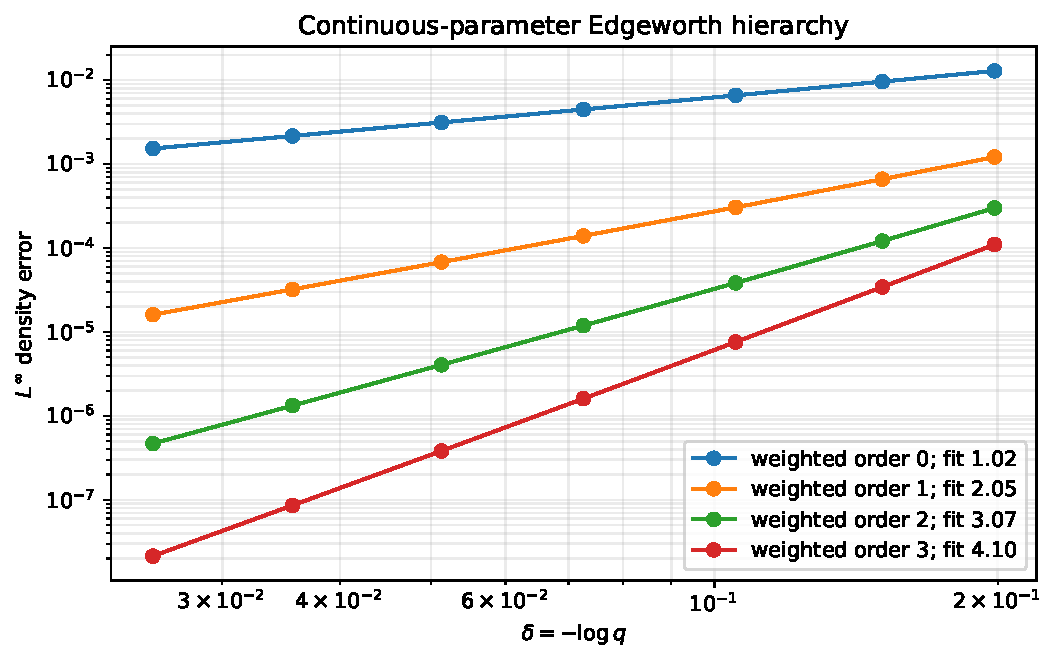
\includegraphics[width=0.92\textwidth]{figures/edgeworth_errors.pdf}
\caption{Sup-norm density errors from direct Fourier inversion.  Fitted
slopes $1.02$, $2.05$, $3.07$, and $4.10$ agree with
\cref{thm:Edgeworth}.}
\label{fig:edgeworth}
\end{figure}

\section{Central, moderate, and large deviations in one scale diagram}
\label{sec:matching}

The Edgeworth and large-deviation results are not separate asymptotic
stories.  The center expansion of $I$ contains the same cumulant information
as the Hermite correction.

Substitute $x=\sigma_qz$ into \eqref{eq:I-center-series} and use
\eqref{eq:variance-delta}.  Uniformly for bounded $z$,
\begin{equation}
 \frac{I(\sigma_qz)}{\delta}
 =\frac{z^2}{2}+\frac{\delta z^4}{20}
 +\delta^2\left(\frac{23z^6}{3150}-\frac{z^2}{24}\right)
 +O\bigl(\delta^3(1+|z|^8)\bigr).
 \label{eq:rate-matching}
\end{equation}
The first exponential correction $\EulerE^{-\delta z^4/20}$ matches the leading
Hermite term $-\delta H_4/20$ after the saddlepoint prefactor is expanded.
The Gaussian moderate-deviation window suggested by the quartic term is
\begin{equation}
 |z|=o(\delta^{-1/4}).
 \label{eq:moderate-window}
\end{equation}
Beyond that scale, the rate function rather than a finite Edgeworth
polynomial becomes the stable description.

\begin{principle}[Three nested regimes]
\label{prin:three-regimes}
As $q=\EulerE^{-\delta}\uparrow1$:
\begin{enumerate}[label=(\roman*)]
\item fixed standardized $z$ is governed by the differentiated Edgeworth
series;
\item $1\ll |z|\ll\delta^{-1/2}$ is governed by the Taylor expansion of
$I(\sigma_qz)/\delta$ and its moderate-deviation resummations;
\item fixed $x\in(-1,1)\setminus\{0\}$ is governed by
$\EulerE^{-I(x)/\delta}$, with Lambert-$W_{-1}$ behavior as $x$ approaches the
support edge.
\end{enumerate}
\end{principle}

\begin{conjecture}[Uniform sharp saddlepoint expansion]
\label{conj:saddlepoint}
For every compact $K\Subset(-1,1)$, the density of $X_{\EulerE^{-\delta}}$ has an
all-orders expansion
\begin{equation}
 f_{X_q}(x)\sim
 \frac{\EulerE^{-I(x)/\delta}}
      {\sqrt{2\pi\delta\Lambda''(\theta_x)}}
 \left(1+\sum_{n\ge1}c_n(x)\delta^n\right),
 \qquad x\in K,
 \label{eq:saddlepoint-conjecture}
\end{equation}
uniformly with all fixed $x$-derivatives.  The coefficients should be
rational differential polynomials in the tilted cumulants
$g^{(k)}(\theta_xe^{-t})$ integrated over $t$.
\end{conjecture}

A proof should combine exponential tilting with a local Edgeworth theorem for
the resulting infinitesimal triangular array.  The midpoint expansion
\eqref{eq:Lambda-two-corrections} implies that no order-one exponential
amplitude is hidden in the finite-$q$ cumulant transform.

\section{Numerical experiments and reproducibility}
\label{sec:numerics}

The archive contains two documented programs.

\begin{itemize}
\item \texttt{experiments.py} performs direct infinite-product Fourier
inversion, midpoint cumulant-transform comparisons, rate-function and
Lambert computations, and a Monte-Carlo stop-loss diagnostic.
\item \texttt{symbolic\_checks.py} uses exact SymPy rational arithmetic to
verify cumulants, Hermite coefficients, the rate series, the kernel cocycle,
and the first Euler--Maclaurin operators.
\end{itemize}

The main numerical outcomes are summarized in \cref{tab:numerical}.

\begin{table}[H]
\centering
\caption{Observed convergence orders and consistency checks.}
\label{tab:numerical}
\begin{tabular}{@{}lr@{}}
\toprule
Quantity & Numerical result \\
\midrule
Uncorrected scaled-CGF order & $1.99999$ \\
After $-\delta^2\theta^2\Lambda''/24$ & $4.00134$ \\
Gaussian density error & $1.01783$ \\
Edgeworth weighted order $1$ & $2.05126$ \\
Edgeworth weighted order $2$ & $3.07181$ \\
Edgeworth weighted order $3$ & $4.09974$ \\
Endpoint constant $\cL$ & $-0.9689204239630311$ \\
Minimum sampled stop-loss gap & $0$ (to displayed precision) \\
Maximum sampled stop-loss gap, $r=.35,s=.72$ & $0.0757670$ \\
\bottomrule
\end{tabular}
\end{table}

\begin{figure}[H]
\centering
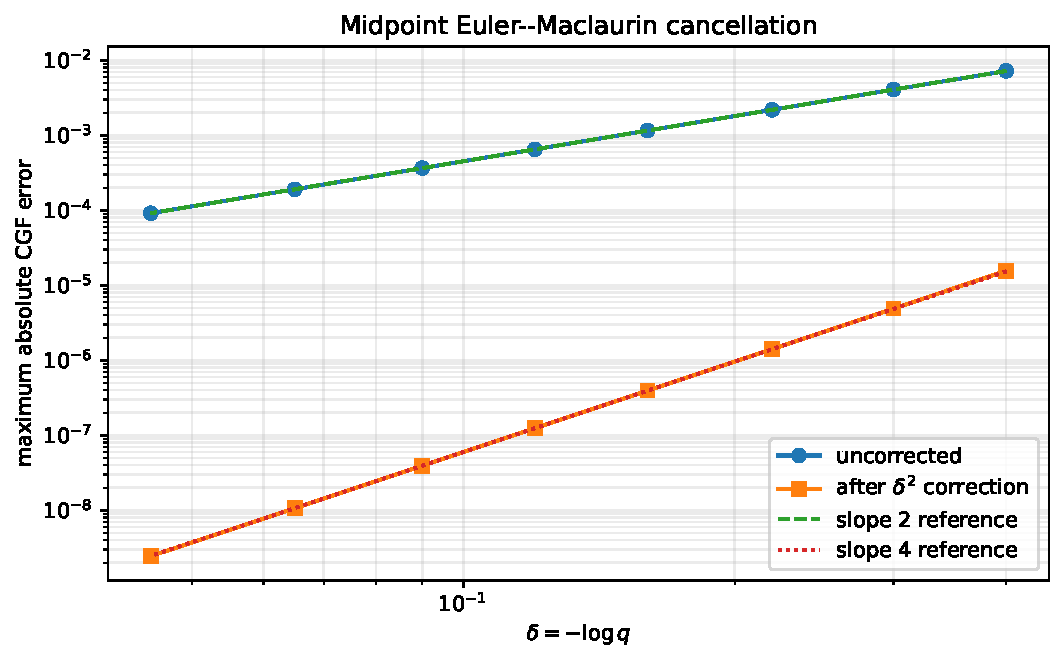
\includegraphics[width=0.92\textwidth]{figures/cgf_midpoint_correction.pdf}
\caption{The raw midpoint-sum error is quadratic in $\delta$; subtracting the
proved first correction exposes the quartic remainder.}
\label{fig:cgf}
\end{figure}

\begin{figure}[H]
\centering
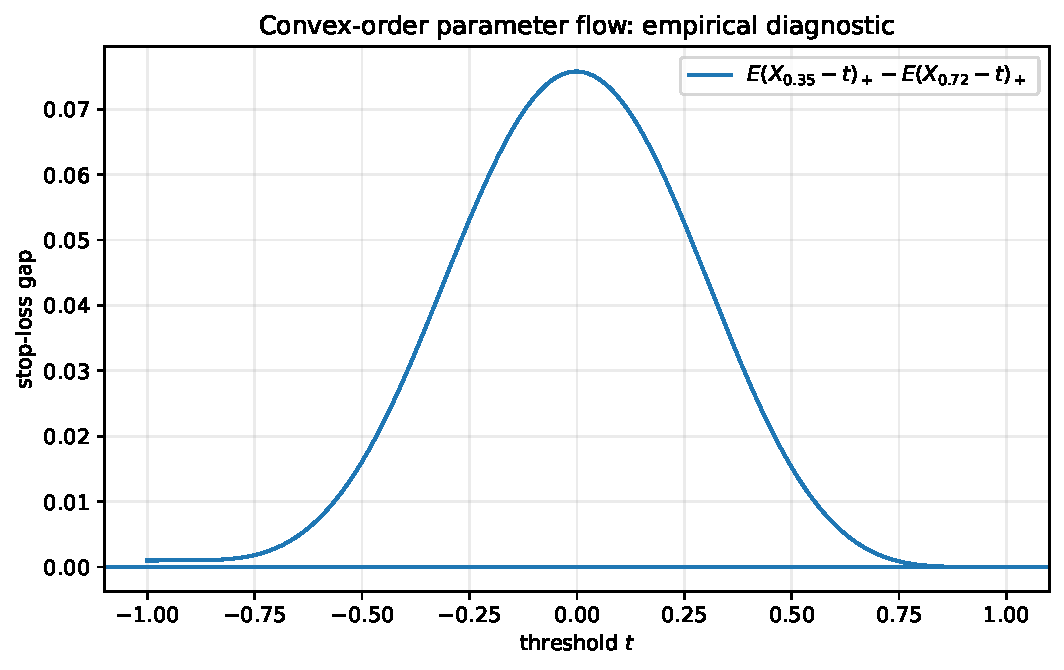
\includegraphics[width=0.92\textwidth]{figures/convex_order_stoploss.pdf}
\caption{Empirical stop-loss gap for two parameter values.  The plot is only
a diagnostic; nonnegativity is proved exactly by the martingale coupling in
\cref{thm:martingale-transport}.}
\label{fig:stoploss}
\end{figure}

\subsection{Numerical methodology}

The standardized density is computed from
\[
 f_q(x)=\frac1\pi\int_0^\infty\chi_q(t)\cos(tx)\Differential t.
\]
The product is truncated only after the first omitted argument is below
$10^{-10}$, and the quadratic logarithmic tail is inserted analytically.  A
cosine quadrature on $[0,30]$ then supplies the density.  The values of
$|\chi_q(30)|$ stored in \texttt{data/edgeworth\_errors.csv} are far below
the reported approximation errors.

The finite-$q$ scaled cumulant transform is evaluated in its exact midpoint
form \eqref{eq:midpoint-sum}.  The endpoint constant is evaluated using the
two absolutely convergent integrals in \eqref{eq:CLambda}.  The stop-loss
experiment uses independent samples and a sorted-sample suffix-sum
algorithm; it is not used in any proof.

\section{Extensions, conjectures, and research program}
\label{sec:future}

\subsection{General bounded seeds}

The two structural results are not special to the uniform law.

\begin{proposition}[Seed-universal transform limit]
\label{prop:general-seed-LDP}
Let $V$ be bounded and let $K_V(\theta)=\log\Expectation \EulerE^{\theta V}$.  For
$X_q^{(V)}$ from \eqref{eq:general-seed},
\begin{equation}
 \delta\log\Expectation\exp\!\left(\frac{\theta X_{\EulerE^{-\delta}}^{(V)}}{\delta}\right)
 \longrightarrow
 \Lambda_V(\theta):=\int_0^\infty K_V(\theta \EulerE^{-t})\Differential t.
 \label{eq:general-seed-Lambda}
\end{equation}
The same midpoint Euler--Maclaurin expansion holds with $g$ replaced by
$K_V$, and the family satisfies a G\"artner--Ellis LDP whenever the limiting
transform is essentially smooth.  Independently, the convex-order flow
\eqref{eq:convex-order} holds for every integrable seed.
\end{proposition}

\begin{proof}
The coefficient identity and martingale proof in \cref{sec:transport} do not
use the distribution of the seed.  For the transform, the exact half-step
calculation gives
\[
 \delta\sum_{j\ge0}K_V(\theta s_\delta \EulerE^{-(j+1/2)\delta}),
\]
and boundedness makes the Riemann-sum and Euler--Maclaurin arguments
uniform.  G\"artner--Ellis applies under its standard regularity hypotheses.
\end{proof}

This suggests a broad ``geometric averaging universality class'' indexed by
the seed cumulant transform.  The uniform seed is distinguished by the
Bernoulli and infinite-sinc structures.

\subsection{Sharp and beyond-all-orders questions}

\begin{conjecture}[Interior all-orders saddlepoint theorem]
The expansion \eqref{eq:saddlepoint-conjecture} is valid and Borel summable
for each fixed compact subinterval of $(-1,1)$.  Its Borel singularities are
governed by the complex zeros of $\sinh z/z$, hence by the same arithmetic
zero lattice that controls the sinc-product Fourier theory.
\end{conjecture}

\begin{conjecture}[Endpoint transseries]
Let $\eta=1-x$ and use the exact Lambert variable
$\theta_0=-W_{-1}(-\eta/2)/\eta$.  The rate and saddle admit full transseries
in inverse powers of $\theta_0$ and exponentials $\EulerE^{-2k\theta_0}$, with no
additional logarithmic scale after $\theta_0$ is adopted.  Matching this
transseries to the finite-$q$ saddlepoint expansion should produce a uniform
double-scaling theory when $\eta$ and $\delta$ tend to zero together.
\end{conjecture}

\begin{problem}[Critical boundary layer]
Determine the correct uniform asymptotics when
\[
 1-x\asymp \delta\log(1/\delta).
\]
This is the scale on which the Lambert saddle
$\theta_x\asymp1/\delta$ meets the largest individual Fourier/MGF argument.
A change of local model, and possibly a Stokes transition, should occur.
\end{problem}

\subsection{Parameter-flow geometry}

The exact shift subordinator invites several extensions.

\begin{problem}[Metric contraction along $q$]
For which probability metrics $d$ does the map $q\mapsto\LawOperator(X_q)$ admit a
closed differential law or sharp contraction coefficient?  Convex order
settles all stop-loss functionals, while the corpus settles several metrics
along finite truncations; the parameter analogue for Wasserstein,
Zolotarev, entropy, and Fisher metrics remains open.
\end{problem}

\begin{conjecture}[Strict stop-loss interior]
For the uniform seed and $0<r<s<1$,
\[
 \Expectation(X_s-t)_+<\Expectation(X_r-t)_+
\]
for every $t\in(-1,1)$.  More generally, the difference should be strictly unimodal in $t$
and inherit a total-positivity property from the random-shift kernel.
\end{conjecture}

\begin{problem}[Generator on laws]
Translate the coefficient jump generator
\[
 \mathcal L_qF(n)=\sum_{k\ge1}q^{k-1}[F(n+k)-F(n)]
\]
into a closed evolution equation for the density or its transform.  The
transform equation is explicit, but a useful physical-space equation may
connect the parameter flow to the Stein--Koopman and diffusion layers already
present in the corpus.
\end{problem}

\subsection{Rate-series arithmetic}

The rational coefficients in \eqref{eq:I-center-series} arise from
compositional inversion of a Bernoulli series.  Their signs, denominators,
and $p$-adic valuations appear to be a new arithmetic sequence.

\begin{problem}[Lagrange--Bernoulli formula]
Find a closed partition formula for the coefficient $c_n$ in
$I(x)=\sum_{n\ge1}c_nx^{2n}$, and determine the exact denominator and
$2$-adic valuation.  A useful formula should expose whether
\cref{conj:rate-positive} follows from a hidden noncrossing, tree, or
continued-fraction interpretation.
\end{problem}

\subsection{Formalization roadmap}

The parameter-flow theorem is especially suitable for formalization:

\begin{enumerate}
\item define the geometric coefficient sequence in $\ell^1$ and prove the
rational generating-function identity;
\item define $p_{r,s}$ and prove positivity, normalization, and cocycle;
\item construct the random shift on an iid sequence and justify exchange of
the two absolutely convergent sums;
\item apply conditional Jensen to obtain convex order;
\item formalize the midpoint identity as an algebraic rewrite before
introducing analytic Euler--Maclaurin estimates.
\end{enumerate}

The LDP and all-order Edgeworth proofs require substantially more analytic
infrastructure.  A practical formal route would first isolate the transform
limit, strict convexity, and the first $O(\delta^2)$ correction; the full
uniform derivative theorem can then be modularized around
\cref{lem:sinc-tail}.

\section{Conclusion}

The geometric-uniform family is more than a deformation that happens to pass
through the Fabius--Rvachev point.  Its coefficient profile carries an exact
probabilistic flow: increasing $q$ is random tail shifting, and random tail
shifting is martingale averaging.  On the analytic side, the same parameter
turns the logarithm of the $q$-product into a midpoint integral.  That single
observation explains the even Euler--Maclaurin hierarchy, produces a new
large-deviation transform, and organizes the continuous Edgeworth expansion.

The resulting picture has three compatible scales.  At the center, Bernoulli
cumulants become Hermite corrections.  At fixed deviations, their integrated
limit becomes a Legendre rate.  At the support edge, the saddle is inverted by
$W_{-1}$.  These layers are distinct from, but structurally aligned with, the
finite-prefix transport, fixed-base endpoint, and discrete $\mathrm{Fup}_n$
results already in the repository.

\appendix

\section{A compact proof ledger}
\label{app:ledger}

For ease of audit, the logical dependencies of the main results are:

\begin{center}
\begin{tabularx}{0.96\textwidth}{@{}lX@{}}
\toprule
Result & Dependencies \\
\midrule
\cref{thm:kernel} & Rational generating functions only \\
\cref{thm:martingale-transport} & \cref{thm:kernel}, iid tail invariance,
conditional Jensen \\
\cref{thm:midpoint-EM} & Exact half-step factorization, midpoint
Euler--Maclaurin, exponential derivative decay \\
\cref{thm:LDP} & \cref{thm:lambda-limit}, compact support,
G\"artner--Ellis \\
\cref{thm:Lambert-edge} & Elementary decomposition of $\log\sinhc$,
$W_{-1}$ inversion \\
\cref{thm:Edgeworth} & Exact cumulants, analytic log-sinc expansion,
\cref{lem:sinc-tail}, Fourier inversion \\
\bottomrule
\end{tabularx}
\end{center}

\section{Explicit rate coefficients through order sixteen}

The symbolic companion gives
\begin{align*}
 I(x)={}&3x^2+\frac95x^4+\frac{276}{175}x^6
 +\frac{1188}{875}x^8+\frac{354672}{336875}x^{10}\\
 &+\frac{1507248}{1990625}x^{12}
 +\frac{496585728}{766390625}x^{14}
 +\frac{53214713856}{65143203125}x^{16}+O(x^{18}),
\end{align*}
and
\begin{align*}
 \theta_x={}&6x+\frac{36}{5}x^3+\frac{1656}{175}x^5
 +\frac{9504}{875}x^7+\frac{709344}{67375}x^9\\
 &+\frac{18086976}{1990625}x^{11}
 +\frac{993171456}{109484375}x^{13}
 +\frac{851435421696}{65143203125}x^{15}+O(x^{17}).
\end{align*}

\section{Files in the reproducibility package}

The ZIP archive contains:
\begin{itemize}
\item \texttt{q\_fabius\_parameter\_frontiers.tex} and the compiled PDF;
\item \texttt{experiments.py}, \texttt{symbolic\_checks.py}, and\linebreak[1] \texttt{requirements.txt};
\item CSV tables for the cumulant-transform, rate, Edgeworth, and stop-loss
experiments;
\item \texttt{numerical\_summary.txt} and
\texttt{symbolic\_checks.txt};
\item the four figures in PDF and PNG formats;
\item a short \texttt{README.md} with reproduction commands.
\end{itemize}

\begin{thebibliography}{99}

\bibitem{Fabius1966}
J.~Fabius,
\newblock A probabilistic example of a nowhere analytic $C^\infty$-function,
\newblock \emph{Z. Wahrscheinlichkeitstheorie verw. Geb.} \textbf{5}
(1966), 173--174.

\bibitem{Rvachev1990}
V.~A.~Rvachev,
\newblock Compactly supported solutions of functional-differential equations
and their applications,
\newblock \emph{Russian Mathematical Surveys} \textbf{45} (1990), no.~1,
87--120; DOI: 10.1070/RM1990v045n01ABEH002324.

\bibitem{Arias2018}
J.~Arias de Reyna,
\newblock Arithmetic of the Fabius function,
\newblock \emph{Integers} \textbf{18} (2018), Paper A51; arXiv:1702.06487.

\bibitem{ProveItDocs}
V.~Reshetnikov,
\newblock ProveIt: FabiusFunction documentation tree,
\newblock \url{https://github.com/VladimirReshetnikov/ProveIt/tree/main/Analysis/FabiusFunction/docs},
accessed 30 August 2026.

\bibitem{ProveItManifest}
V.~Reshetnikov,
\newblock Draft manifest for the semi-formalized Fabius--Rvachev research
frontiers,
\newblock \url{https://github.com/VladimirReshetnikov/ProveIt/blob/main/Analysis/FabiusFunction/docs/semi-formalized-research-frontiers/drafts/MANIFEST.md},
accessed 30 August 2026.

\bibitem{Corless1996}
R.~M.~Corless, G.~H.~Gonnet, D.~E.~G.~Hare, D.~J.~Jeffrey, and D.~E.~Knuth,
\newblock On the Lambert $W$ function,
\newblock \emph{Advances in Computational Mathematics} \textbf{5} (1996),
329--359.

\bibitem{Ellis1984}
R.~S.~Ellis,
\newblock Large deviations for a general class of random vectors,
\newblock \emph{Annals of Probability} \textbf{12} (1984), 1--12.

\bibitem{DemboZeitouni}
A.~Dembo and O.~Zeitouni,
\newblock \emph{Large Deviations Techniques and Applications},
\newblock 2nd ed., Springer, 1998; corrected printing 2010.

\bibitem{BhattacharyaRao}
R.~N.~Bhattacharya and R.~Rao,
\newblock \emph{Normal Approximation and Asymptotic Expansions},
\newblock Wiley, 1976; SIAM Classics reprint, 2010.

\bibitem{Petrov}
V.~V.~Petrov,
\newblock \emph{Sums of Independent Random Variables},
\newblock Springer, 1975.

\bibitem{MarshallOlkinArnold}
A.~W.~Marshall, I.~Olkin, and B.~C.~Arnold,
\newblock \emph{Inequalities: Theory of Majorization and Its Applications},
\newblock 2nd ed., Springer, 2011.

\bibitem{HardyLittlewoodPolya}
G.~H.~Hardy, J.~E.~Littlewood, and G.~P\'olya,
\newblock \emph{Inequalities},
\newblock 2nd ed., Cambridge University Press, 1952.

\bibitem{Olver}
F.~W.~J.~Olver,
\newblock \emph{Asymptotics and Special Functions},
\newblock Academic Press, 1974; A K Peters reprint, 1997.

\bibitem{GasperRahman}
G.~Gasper and M.~Rahman,
\newblock \emph{Basic Hypergeometric Series},
\newblock 2nd ed., Cambridge University Press, 2004.

\bibitem{Comtet}
L.~Comtet,
\newblock \emph{Advanced Combinatorics: The Art of Finite and Infinite
Expansions},
\newblock Reidel, 1974.

\end{thebibliography}

\end{document}
